\documentclass[10pt,a4paper]{article}
\usepackage[utf8]{inputenc}
\usepackage[italian]{babel}
\usepackage{amsmath}
\usepackage{amsfonts}
\usepackage{amssymb}
\usepackage{graphicx}
\usepackage[left=2cm,right=2cm,top=2cm,bottom=2cm]{geometry}
\newcommand{\rem}[1]{[\emph{#1}]}

\author{Gruppo AC \\ Federico Belliardo, Giulia Franchi, Francesco Mazzoncini}
\title{Esercitazione N.1: Misure di tensione, corrente, tempi, frequenza.}
\begin{document}

\maketitle

\section{Scopo e strumentazione}

L'esercitazione ha lo scopo di impratichirsi con la strumentazione e le tecniche di misura. 
Abbiamo utilizzato sia il multimetro digitale sia il tester analogico. 

\section{Misure di tensione e corrente}
\paragraph{2.b Partitore}
Abbiamo montato il circuito in Fig. 1 con i valori di resistenza misurati con il multimetro digitale: $R_1 = 0,99\pm 0.01 k\Omega$ e $R_2 = 0.99\pm 0.01 k\Omega$. L'errore \`e stato stimato usando le indicazioni del manuale del multimetro ($0.8\%$ + 1 cifra). 
Dall'analisi del circuito ci aspettiamo che $V_\mathrm{OUT}/V_\mathrm{IN} = \frac{1}{1+R_1/R_2}= 0.501 \pm 0.003 $.


Variando $V_\mathrm{IN}$ tra 0 e 10V abbiamo ottenuto i dati riportati in Tabella~\ref{t:par1} e Figura~\ref{f:par1}.

\begin{table}[h]
\centering
\begin{tabular}{|c|c|c|c|c|c|}
\hline 
VIN& $\sigma$ VIN  &VOUT	 & $\sigma$ VOUT& VOUT/VIN & $\sigma$ VOUT/VIN \\
\hline 
1.84&0.01&0.95&0.01&0.516&0.005\\
3.24&0.02&1.63&0.01&0.503&0.003\\
4.10&0.02&2.05&0.01&0.500&0.002\\
6.04&0.03&3.03&0.02&0.502&0.003\\
7.08&0.04&3.55&0.02&0.501&0.003\\
8.61&0.04&4.31&0.02&0.501&0.002\\
9.88&0.05&4.95&0.03&0.501&0.003\\
\hline 
\end{tabular} 
\caption{Partitore di tensione con resistenze da circa 1k. Tutte le tensioni in V.\label{t:par1}}
\end{table}
\begin{figure}
\centering
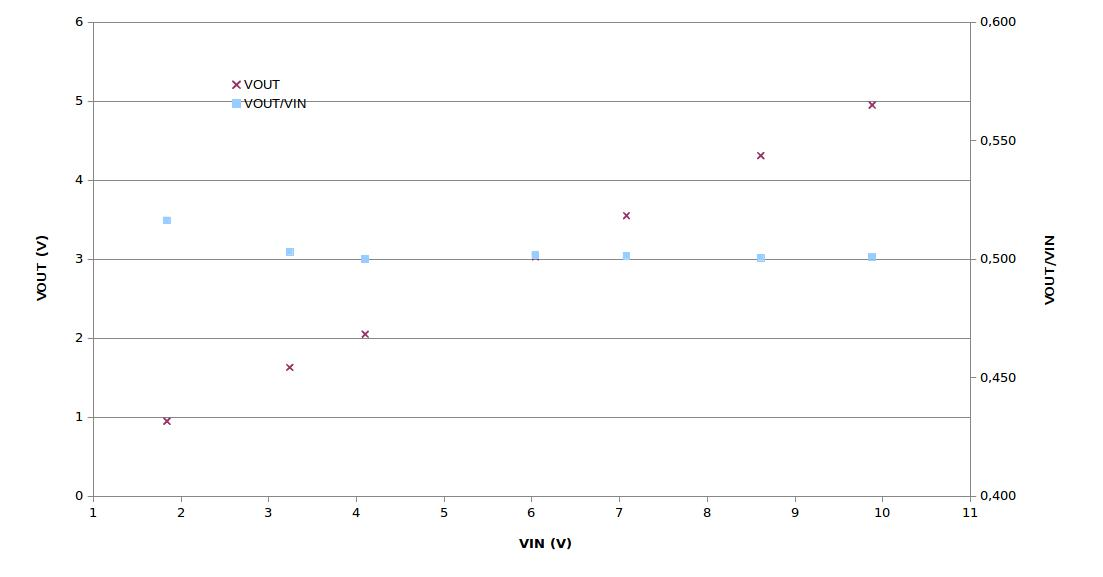
\includegraphics[scale=0.6]{part1.jpg}
\caption{Partitore di tensione con resistenza da circa 1k.\label{f:par1}}
\end{figure}
Come ci si aspettava la relazione tra tensione di ingresso ed uscita \`e lineare. Il rapporto VOUT/VIN \`e da confrontare con il valore aspettato indicato sopra.

Gli errori sulle tensioni e sul loro rapporto sono stati calcolati con la formula della somma in quadratura.
 
%\rem{Volendo si pu\`o fare la media pesata dei valori misurati }

\paragraph{2.c Partitore con resitenze pi\`u grandi}
Montando di nuovo il partitore con le resistenze $R_1 = 5.03\pm 0.05 M\Omega$ e $R_2 = 3.56\pm 0.04 M\Omega$ si osservano i nuovi dati in Tabella~\ref{t:par2} e Figura~\ref{f:par2}
\begin{table}[h]
\centering
\begin{tabular}{|c|c|c|c|c|c|c|c}
\hline 
VIN& $\sigma$ VIN  &VOUT	 & $\sigma$ VOUT& VOUT/VIN & $\sigma$ VOUT/VIN& $\frac{R_{1}}{R_{T}}$ & $\sigma \frac{R_{1}}{R_{T}}$ \\
\hline 

1.99&0.01&0.680&0.007&0.342&0.005&0.51&0.01\\
2.02&0.02&0.87&0.01&0.342&0.003&0.51&0.01\\
2.99&0.03&1.26&0.02&0.344&0.003&0.49&0.01\\
3.95&0.04&1.68&0.02&0.343&0.004&0.50&0.01\\
5.01&0.05&2.14&0.02&0.343&0.003&0.50&0.01\\
7.50&0.08&3.20&0.03&0.347&0.004&0.47&0.01\\
10.02&0.10&4.28&0.03&0.344&0.004&0.49&0.01\\
\hline 
\end{tabular} 
\caption{Partitore di tensione. Tutte le tensioni in V.\label{t:par2}}
\end{table}
\begin{figure}[h]
\centering
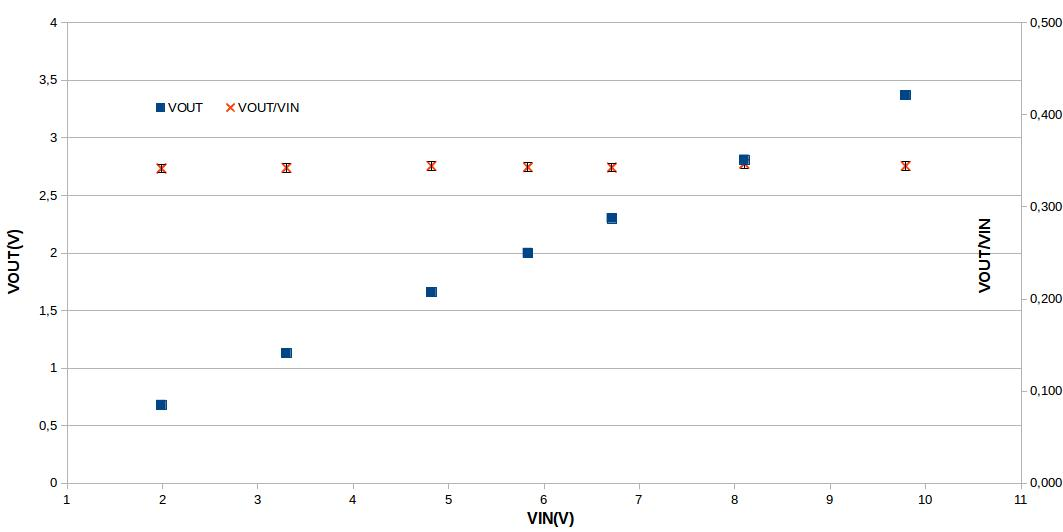
\includegraphics[scale=0.6]{part2.jpg}
\caption{Partitore di tensione con resistenze da circa 4M.\label{f:par2}}
\end{figure}

Si può calcolare il valrore medio di $V_\mathrm{OUT}/V_\mathrm{IN}$ ottenendo $V_\mathrm{OUT}/V_\mathrm{IN} = 0.343 \pm 0.005$.
Si osserva come valore del rapporto misurato con le resistenze da $4~M\Omega$ si discosti da quanto atteso   $V_\mathrm{OUT}/V_\mathrm{IN} = \frac{1}{1+R_1/R_2}= 0.414\pm 0.003 $. La ragione della discrepanza \`e da ricercarsi nella impedenza di ingresso del tester.


\paragraph{2.d Resistenza di ingresso del tester}

 Usando il modello mostrato nella scheda si ottiene
\[ \frac{R_1}{R_T} =  \frac{V_{IN}}{V_{OUT}} - (1 +  \frac{R_1}{R_2} )
\]
L'errore sul secondo membro \`e: 1.4\% sul primo termine, 0.7\% sul secondo termine. Entrambi i termini sono circa 2, per cui l'errore totale \`e $ 0.03 \oplus 0.015 = 0.035$, dominato dalla misura di tensione. Quindi se  $R_T > R_1/0.035 $ non abbiamo nessuna sensibilit\`a sperimentale. 
Nel seguito sono riportati in talella i valori misurati del rapporto $R_1/R_T$ per ogni tensione.


Nel primo caso risulta un numero compatibile con 0: usando la media del rapporto VOUT/VIN, abbiamo $R_1/R_T = -0.01 \pm 0.03 $.
Nel secondo caso risulta invece $R_1/R_T =0.50 \pm 0.02 $ cio\`e $ R_T = 10.1 \pm 0.5 M\Omega$.

\subsection{Partitore di corrente: 2.e}

Si monta il circuito indicato con i valori di resistenza misurati con il multimetro digitale: 
$R_3= 100\pm 2 k\Omega$, $R_1 = 548\pm 5 \Omega$, $R_2 = 217\pm 3 \Omega$.
Si fissa la tensione dell'alimentatore a $V_{IN}=10.00 \pm 0.05 V$ e si utilizza il tester digitale per misurare alternativamente la corrente nel ramo 1 e nel ramo 2, sostitendo il ramo non sotto misura con un cortocircuito. 


Si ottengono le seguenti misure: $I1 = 25 \pm 1 \mu ~A $, $I2 = 63 \pm 1 \mu ~A $. 
Si ripetono le misure utilizzando il tester analogico, e si ottengono i seguenti valori:
$I1 = 7.0 \pm 0.5 \mu A $, $I2 = 18 \pm 1 \mu ~A $. 
Ci si aspetterebbe che il rapporto tra le correnti sia $I1/I2 = R2/R1 = 0.418 \pm 0.006$ e che la somma delle correnti sia $I1 + I2 = I_{TOT} \equiv V_{IN}/R3 = 97 \pm 2 \mu~A$, considerando che l'approssimazione $I_{TOT}=V_{IN}/R3$ vale quando $R3>>$altre resistenze in gioco, ed \`e certamente verificata in questo circuito. 
Tuttavia si nota che i valori effettivamente misurati con il tester analogico ed il tester digitale si discostano da tali valori:

\begin{center}
\begin{tabular}{|c|c|c|c|c|c|c|c|c|}
\hline 
strumento& I1 ($\mu A$)& $\sigma$(I1) ($\mu A$) & I2	($\mu A$) & $\sigma$(I2) ($\mu A$) & I1/I2 
& $\sigma$(I1/I2) & I1+I2 & $\sigma$(I1+I2) \\
\hline 
Analogico & 7.0 & 0.5  & 18 & 1 & 0.39 & 0.05 & 25 & 2 \\
Digitale & 25 & 1  & 63 & 1 & 0.40 & 0.02 & 88 & 2 \\
\hline 
\end{tabular} 
\end{center}

%Eseguire eventualmente solo una misura con analogicoo digitale%

La discrepanza tra  nasce dalla resistenza interna dell'amperometro che altera la resistenza lungo ciascun ramo quando viene inserito. 
Detta $R_A$ la resistenza dell'amperometro,
questa viene sommata alternativamente ad $R1$ oppure $R2$, per cui $I1/I2 = (R2+R_A)/(R1+R_A)$ 
e $I1+I2 = I_{TOT}\cdot(R1+R2)/(R1+R2+R_A)$.
Si pu\`o quindi stimare 
$$
R_A = (R1+R2)\left(\frac{I_{TOT}}{I1+I2} - 1 \right)
$$

Per l'amperometro digitale si ottiene: $R_A = 0.17 \pm 0.07 k\Omega$, per quello analogico otteniamo invece $R_A = 1.6 \pm 0.2 k\Omega$. La misura della resistenza interna dell'amperometro analogico risulta evidentemente troppo alta per essere realistica.  

\section{Uso dell'oscilloscopio}

\paragraph{Misure di tensione}

Eseguo tre misure di tensione in accoppiamento DC e AC (riportate in Tabella~\ref{t:par3}). 
Le misure in tabella riportano soltanto il valore di $V_{IN}$ e $V_{OUT}$ in accoppiamento DC, le misure effettuate in accoppiamento AC sono risultate tutte a zero.

\begin{table}[h]
\centering
\begin{tabular}{|c|c|c|c|}
\hline 
VIN &  $\sigma$ VIN & VOUT &  $\sigma$ VOUT\\

\hline 

11.00&0.01&5.52&0.01\\

\hline 
\end{tabular} 
\caption{Misure nei due accoppiamenti dell'oscilloscopio.\label{t:par3}}
\end{table}

In corrente continua passare all'accoppiamento AC annulla il segnale sull'oscilloscopio. 

\paragraph{Impedenza di ingresso dell'oscilloscopio}

Per valutare l'impedenza di ingresso dell'oscilloscopio (Figura ~\ref{t:par4})  lo si collega in serie ad un amperometro. Con la caduta di potenziale dall'oscilloscopio e la misura dell'intensità di corrente otteniamo la resistenza totale del circuito, dalla quale otteniamo una stima dell'impedenza interna dell'oscilloscopio. Si sono misurati: $V = 10.1 \pm 0.3V$ e $I = 8 \pm 1 \muA$, per cui $R_i = V/I = 1,3 \pm 0,2 M\Omega$.
In questo si trascura la resistenza interna del generatore e dell'amperometro (esse sono nell'ordine delle decine di Ohm)

\begin{figure}
\centering
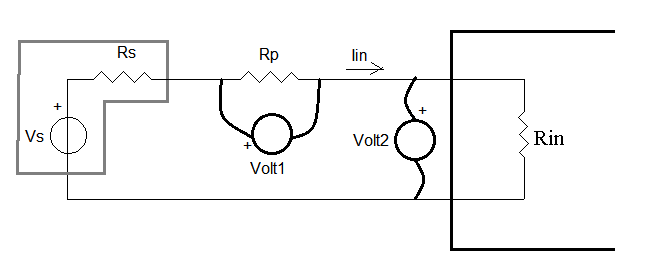
\includegraphics[scale=0.8]{resistenzaIngresso.png}
\caption{Schema circuitale per la misura dela resistenza di ingresso\label{t:par4}}
\end{figure}


\section{Misure di frequenza e tempo}

Nella Tabella~\ref{t:par5} sono riportate le misure di frequenza utilizzando la scala graduata e utilizzando la funzione dell'oscilloscopio.
\begin{table}[h]
\centering
\begin{tabular}{|c|c|c|}
\hline 
Frequenza (kHz) & Scala graduata (kHz) & Funzione strumento (kHz) \\

\hline 

1&$ 0.97 \pm 0.01$  &0.98\\
10& $10.4 \pm 0.2$ &10.3\\
100& $101 \pm 1$ &101.97\\
1000& $1040 \pm 5$ &1029\\

\hline 
\end{tabular} 
\caption{Misure di frequenza.\label{t:par5}}
\end{table}

L'errore sulle sulle misure di fequenza ricavate dalla scala dei tempi sono state ottenute propagando l'errore di musura sulla scala graduata dei tempi. Non sono stati riportati invece gli errori relativi al frequenzimetro interno dell'oscilloscopio perchè questo valore è calcolato dall'oscilloscopio per mezzo di un algoritmo a "scatola chiusa".

Di seguito sono riportate le misure del tempo in cui il segnale è rispettivamente positivo e nullo per diversi duty-cycle con i relativi screenshoot: duty-cycle a $10\% \rightarrow $ 460 ms e 4600 ms, $50\% \rightarrow $ 480 ms e 990 ms, $90\% \rightarrow$ 4800 ms e 480 ms.


\begin{figure}
\centering
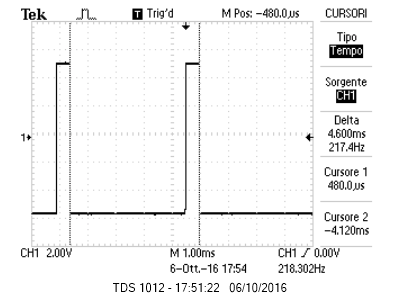
\includegraphics[scale=0.8]{dutycicle10_.png}
\caption{Duty-cycle al 10$\%$}
\end{figure}

\begin{figure}}[h]
\centering
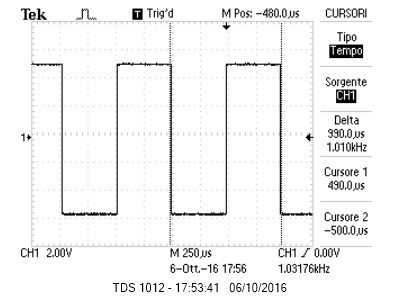
\includegraphics[scale=0.8]{dutycicle50_.png}
\caption{Duty-cycle al 50$\%$}
\end{figure}

\begin{figure}}[h]
\centering
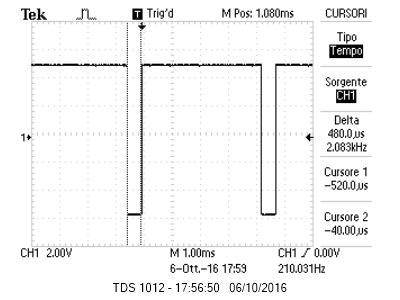
\includegraphics[scale=0.8]{dutycicle90_.png}
\caption{Duty-cycle al 90$\%$}
\end{figure}


\section{Trigger dell'oscilloscopio}

Il pulse e l'onda quadra saranno sfasati temporalmente: per l'onda quadra vi è uno sfasamento di $\frac{\pi}{2}$; per l'onda sinusoidale il pulse si accende quando l'onda è al suo massimo, mentre al minimo si spegne; per l'onda triangolare invece al massimo si spegne e al minimo si accende.

Le figure riguardanti il segnale di pulse alla fine del decumento giustificano le affermazioni precedenti.

Le figure seguenti riportano l'ampiezza del segnale per oscillazione a un $MHz$:

\begin{figure}
\centering
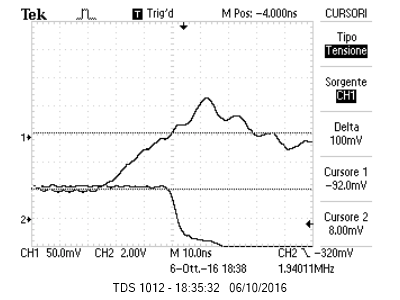
\includegraphics[scale=0.8]{ampiezza_segnale.png}
\caption{Ampiezza del segnale - fase di salita}
\end{figure}


\begin{figure}
\centering
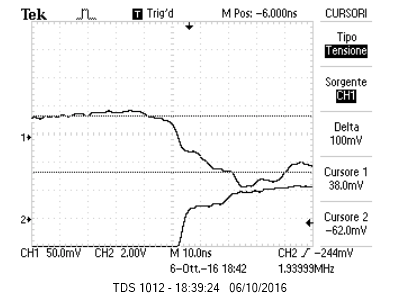
\includegraphics[scale=0.8]{discesa.png}
\caption{Ampiezza del segnale - fase di discesa}
\end{figure}

Riporto nella Tabella~\ref{t:par6} per salita e discesa corrispondenti al 10\% e al 90\% del segnale, misurati utilizzando i cursori e stimati dall'oscilloscopio. Nuovamente non conosciamo l'algoritmo per il calcolo del tempo di salita e ci limitiamo a riportarlo senza errore.
 
Il segnale vale: $V_{signal} = 100 \pm 10 mV$, quindi il 10\% e il 90\% sono:
$V_{10} = 10 \pm 1 mV $ e $V_{90} = 90 \pm 9 mV$. 

\begin{table}[h]
\centering
\begin{tabular}{|c|c|c|}
\hline 
Zona & Cursori (ns) & Oscilloscopio (ns) \\
\hline 
Salita&$21.6 \pm 0.2 $& 33\\
Discesa&$14.8 \pm 0.2$& 29\\
\hline 
\end{tabular} 
\caption{Misure di tempo.\label{t:par6}}
\end{table}

\begin{figure}}[h]
\centering
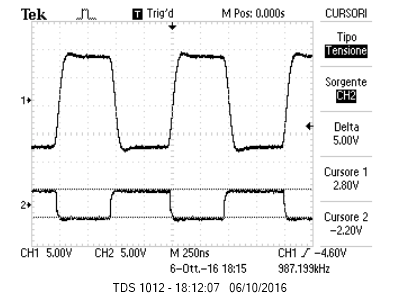
\includegraphics[scale=0.8]{pulsequadra.png}
\caption{Onda quadra}
\end{figure}

\begin{figure}}[h]
\centering
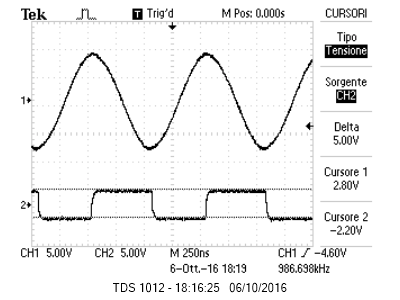
\includegraphics[scale=0.8]{pulsesinus.png}
\caption{Onda sinusoidale}
\end{figure}

\begin{figure}[h]
\centering
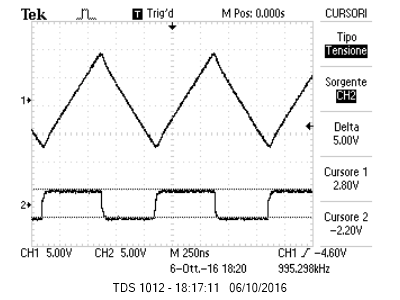
\includegraphics[scale=0.8]{pulsetriang.png}
\caption{Onda triangolare}
\end{figure}

\section{Conclusioni e commenti finali}
Non siamo risuciti a capire perchè le misure di corrente con l'amperometro analogico diano risultati così discordanti da quelli attesi.

\end{document}